\section{Introduction: Dyson-Schwinger Equations, Spectral Representations}

\begin{frame}{Real-time Formulation of QFT}
\addtocounter{framenumber}{-1}
\begin{itemize}
	\item Application of \alert{non-perturbative} techniques (FRG, DSE, lattice): Usually \alert{Euclidean} expressions\\[1em]
	\item If we want to access \alert{dynamical properties} $\rightarrow$ Need \alert{real-time} quantities!\\[1em]
\end{itemize}
\vfill
\alert{Is there a (simple) possibility to get access to the respective real-time quantities?}
\vfill
\begin{itemize}
	\item Problem: Map from $\mathbb{R}^4$ to Minkowski space is non-trivial! \\[1em]
	\item Need \alert{Numerical reconstruction techniques} or access to \alert{algebraic momentum structure}!
\end{itemize}



\end{frame}

\begin{frame}{Dyson-Schwinger Equations}
\begin{itemize}
	\item From \alert{shift symmetry} of the path integral measure, the \alert{master DSE} can be derived:
\end{itemize}
\begin{equation}
\frac{\delta \Gamma[\phi]}{\delta \phi(x)}=\frac{\delta S[\phi]}{\delta \varphi(x)}\left[\varphi=G \cdot \frac{\delta}{\delta \phi}+\phi\right] \label{eqn:DSE}
\end{equation}
\begin{itemize}
	\item Higher correlation functions are obtained by taking functional derivatives: $\left(\frac{\delta}{\delta\phi}\right)^n$
\end{itemize}
\begin{figure}[t]
	\centering
	\begin{align*}
	\hspace{-25 pt} 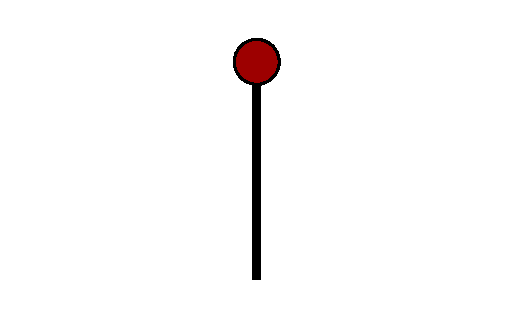
\includegraphics[scale=0.4, valign=c]{figs/diagrams/masterDSE/d_gamma} \hspace{-30 pt}=\hspace{-30 pt} 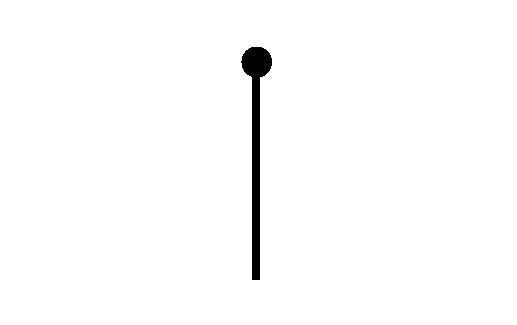
\includegraphics[scale=0.4, valign=c]{figs/diagrams/masterDSE/d_S} \hspace{-30 pt}+\hspace{20pt}\mathlarger{\frac{1}{2}} \hspace{-20 pt}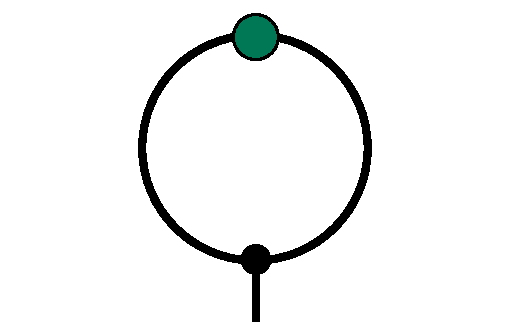
\includegraphics[scale=0.4, valign=c]{figs/diagrams/masterDSE/one_loop} \hspace{-20 pt}-\hspace{20pt} \mathlarger{\frac{1}{6}} \hspace{-20 pt}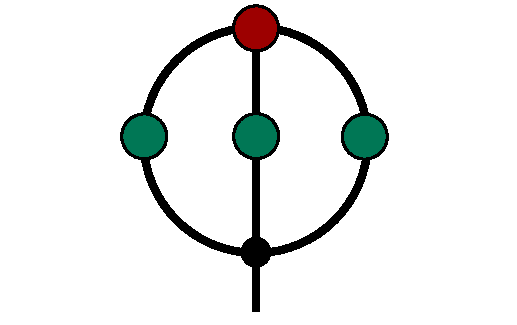
\includegraphics[scale=0.4, valign=c]{figs/diagrams/masterDSE/two_loop}
	\end{align*}
	\caption{Diagrammatic representation of the master DSE in scalar theory}\label{fig:masterDSE_scalar}
\end{figure}
\end{frame}

\begin{frame}{K\"all\'{e}n-Lehmann Spectral Representation of Correlation Functions}
\begin{itemize}
	\item Spectral representation of the (scalar) propagator:
\end{itemize}
\begin{align} 
G(p)=\int_{0}^{\infty} \frac{\dd \lambda^2}{\pi} \frac{\rho(\lambda^2)}{p^{2}+\lambda^{2}}. \label{eqn:KL_rep}
\end{align}
\begin{itemize}
	\item Inverse relation between spectral function $\rho$ and (retarded) propagator:
\end{itemize}
\begin{equation}
	\rho(\omega, \abs{\mathbf{p}}) = 2 \operatorname{Im}\left[G\left(-i(\omega + i0^+), \abs{\mathbf{p}}\right)\right]. \label{eqn:specfunc_relation}
\end{equation}
\begin{itemize}
	\item Spectral reps. for higher order correlators should exist from axiomatic viewpoint. \\ \alert{Here:} Classical vertex approximation!
\end{itemize}


\end{frame}

\begin{frame}{Example: Scalar Theory}
\begin{figure}
	\centering
	\hspace{-2em}
	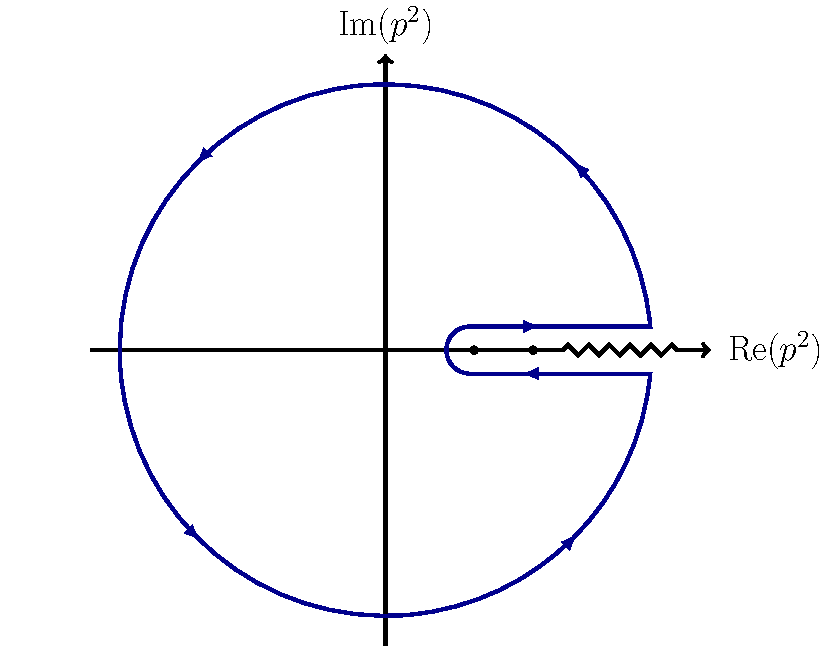
\includegraphics[width=0.43\textwidth]{figs/tikz/contour}
	\hspace{2em}
	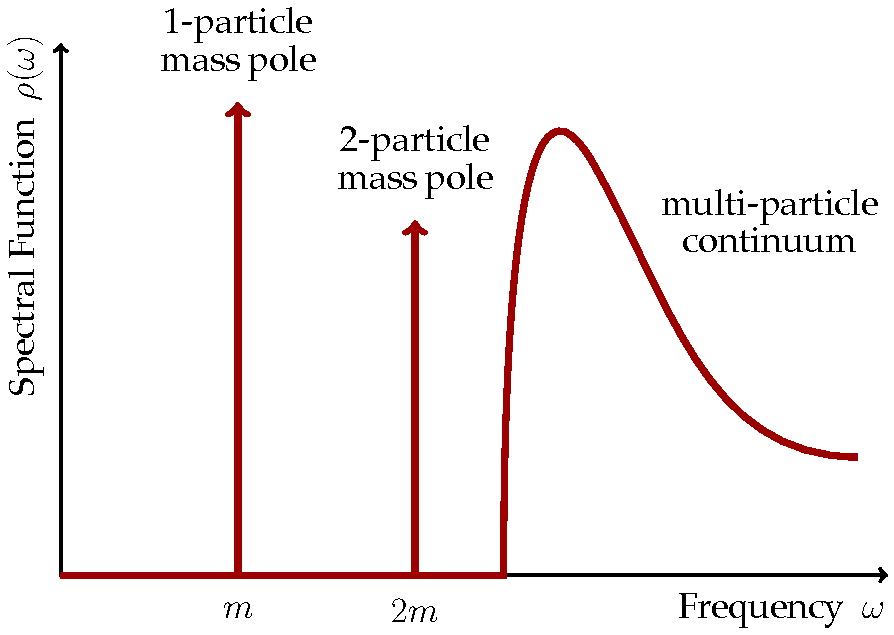
\includegraphics[width=0.43\textwidth]{figs/tikz/scalar_spec_func}\label{fig:scalar_spec_func}
	\caption{\textit{Left:} Analytic Structure of a scalar propagator with respective integration contour in the complex plane. \textit{Right:} Shape of the associated spectral function.}
\end{figure}
\end{frame}


\begin{frame}{Relevant DSEs for QCD Propagators}
\begin{figure}[H]
\centering
\begin{align*}
\bigg(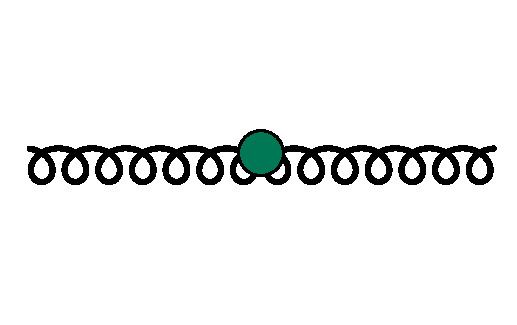
\includegraphics[scale=0.3, valign=c]{figs/diagrams/gluonDSE/full_gluon_propagator}\bigg)^{-1} &= 
\bigg(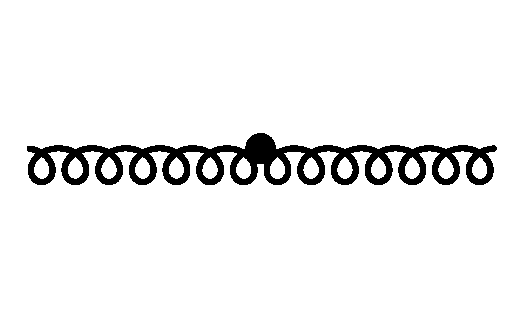
\includegraphics[scale=0.3, valign=c]{figs/diagrams/gluonDSE/bare_gluon_propagator.pdf}\bigg)^{-1}\ - \frac{1}{2}\ 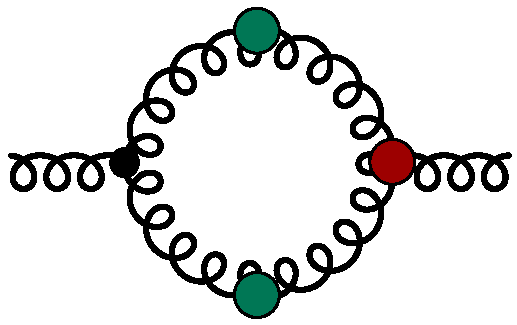
\includegraphics[scale=0.3, valign=c]{figs/diagrams/gluonDSE/gluon_polarization}\ +\ \frac{1}{2}\ 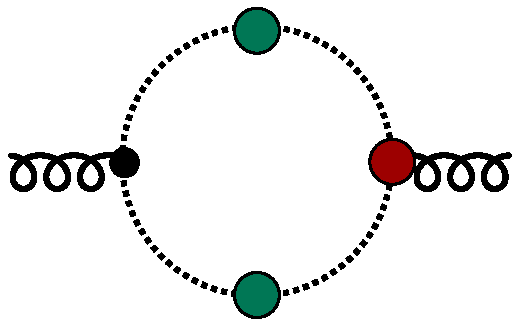
\includegraphics[scale=0.3, valign=c]{figs/diagrams/gluonDSE/ghost_polarization}  \\[0.8em]
\bigg(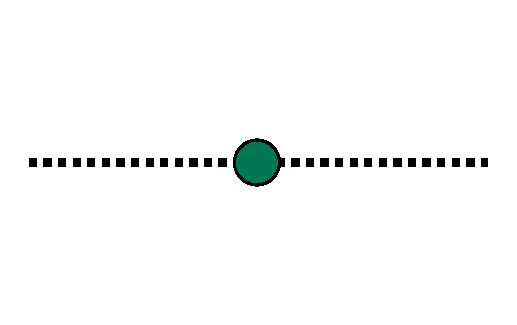
\includegraphics[scale=0.3, valign=c]{figs/diagrams/ghostDSE/full_ghost_propagator}\bigg)^{-1} &= 
\bigg(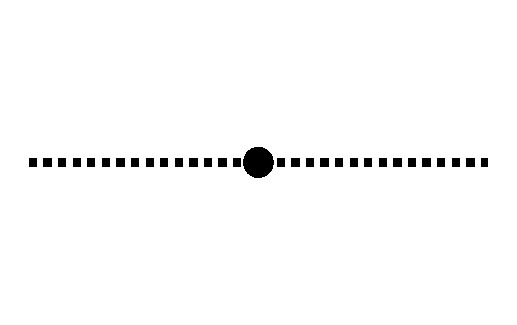
\includegraphics[scale=0.3, valign=c]{figs/diagrams/ghostDSE/bare_ghost_propagator.pdf}\bigg)^{-1}\hspace{0.625em} -\hspace{0.625em}   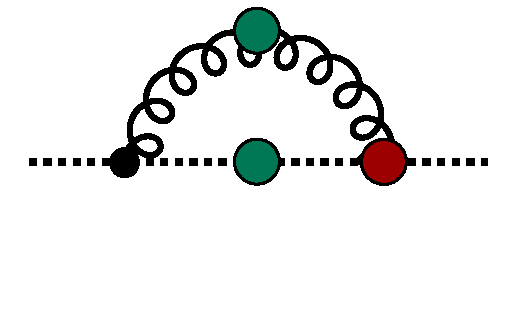
\includegraphics[scale=0.3, valign=c]{figs/diagrams/ghostDSE/ghost_self_energy} \\[0.8em]
\bigg(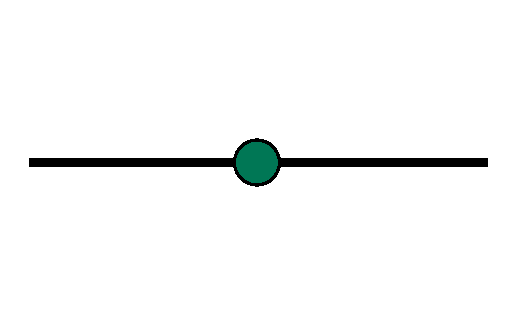
\includegraphics[scale=0.3, valign=c]{figs/diagrams/quarkDSE/full_quark_propagator}\bigg)^{-1} &= 
\bigg(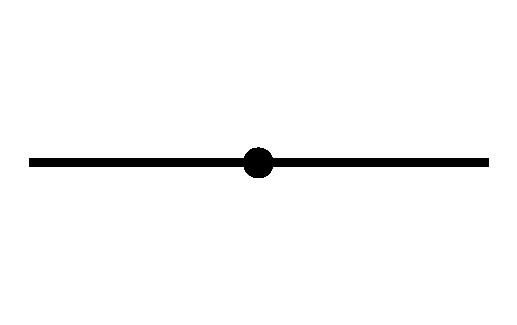
\includegraphics[scale=0.3, valign=c]{figs/diagrams/quarkDSE/bare_quark_propagator.pdf}\bigg)^{-1}\hspace{0.625em} -\hspace{0.625em} 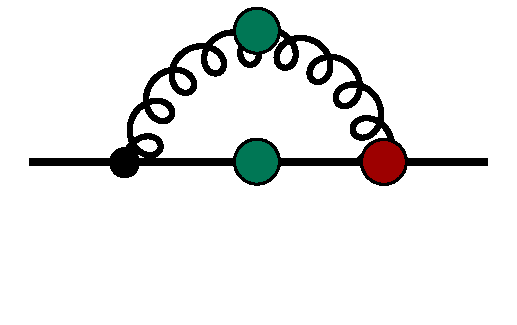
\includegraphics[scale=0.3, valign=c]{figs/diagrams/quarkDSE/quark_self_energy}
\end{align*}

\caption{\textit{Top row:} Gluon DSE, truncated at one-loop. \textit{Middle row:} Ghost DSE. \textit{Bottom row:} Quark DSE.}
\end{figure}
\end{frame}

\begin{frame}{Quark Self Energy Diagram}
\begin{itemize}
	\item Assuming classical vertices, the nontrivial contribution to the quark DSE reads:
\end{itemize}
\begin{align}
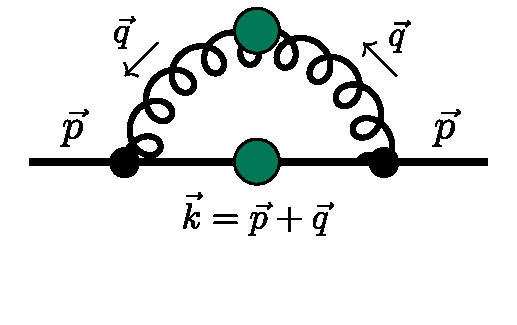
\includegraphics[scale=0.45, valign=c, trim = 0 6em 0 0]{figs/diagrams/quark_self_energy_classical} := \Sigma_q
(p) &= (-ig)^2 \delta^{ab}C_f \int_q\ \Pi^{\mu\nu}_{\perp}(q) G_A(q)\gamma_{\mu}G_q(p+q)\gamma_{\nu}.
\end{align}
\begin{itemize}
	\item Insert spectral representations for gluon and quark propagators
\end{itemize}
\begin{align}
G_{A}(q)&= \int_{\lambda_1}\ \frac{\lambda_1\rho_A(\lambda_1)}{q^{2}+\lambda_1^{2}},\label{eqn:GluonSpec}\\[1em]
G_q(p+q) &= -i(\slashed{p}+\slashed{q})\left(\frac{Z_q(p)}{p^2 + M_q^2(p)}\right) +  \left(\frac{Z_q(p)M_q(p)}{p^2 + M_q^2(p)}\right)\nonumber \\
&= (\slashed{p}+\slashed{q}) \int_{\lambda_2}\ \frac{\lambda_2\rho_{q}^D(\lambda_2)}{(p+q)^{2}+\lambda_2^2}+ \int_{\lambda_2}\ \frac{\lambda_2\rho_{q}^M(\lambda_2)}{(p+q)^{2}+\lambda_2^2}.\label{eqn:QuarkSpecFunc}
\end{align}


\end{frame}

\section{Methodology: Spectral Renormalization Scheme}

\begin{frame}{Spectral Renormalization Scheme: Overview}
\addtocounter{framenumber}{-1}
 \begin{figure}[t]
\centering
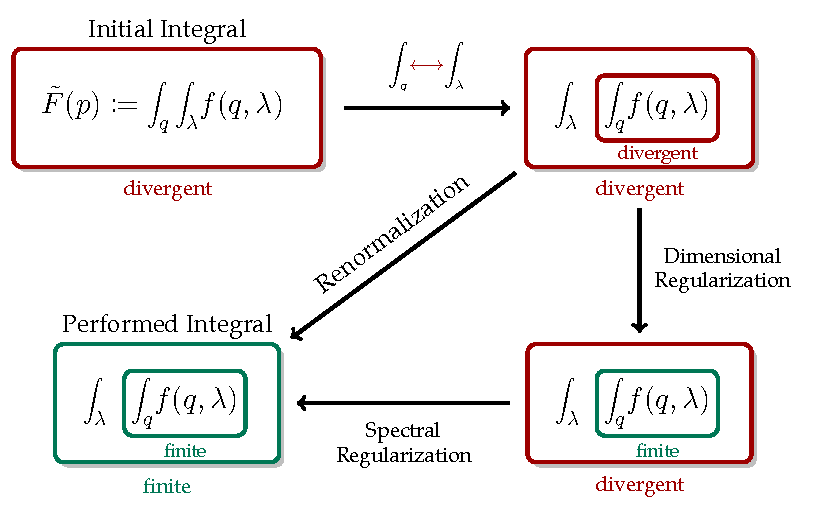
\includegraphics[width=0.8\textwidth]{figs/tikz/spectral_renormalization}
\end{figure}
\end{frame}

\begin{frame}{BPHZ-type Subtraction Scheme for the Spectral Integrands}
\begin{itemize}
	\item Remnant of swapping integration order: we are not done after \alert{Dimensional Regularization}!
\end{itemize}
	 \begin{figure}[H]
	\centering
	\begin{align*}
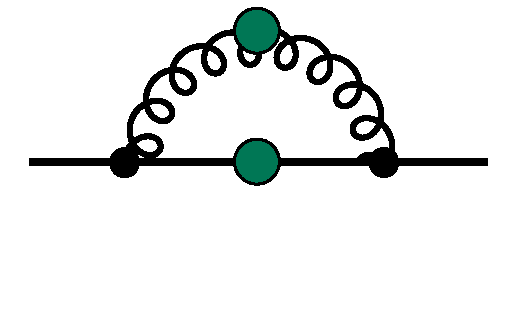
\includegraphics[scale=0.28, valign=c]{figs/diagrams/bphz/quark_self_energy_classical} \longrightarrow 
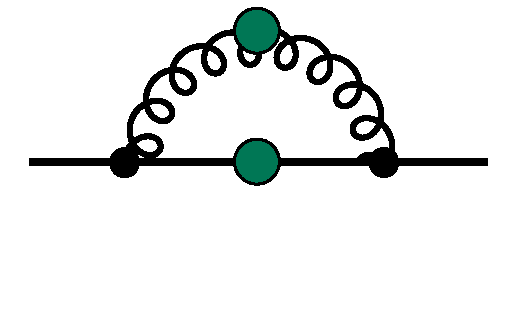
\includegraphics[scale=0.28, valign=c]{figs/diagrams/bphz/quark_self_energy_classical} - \eval{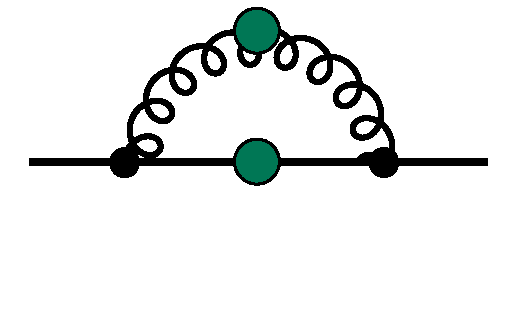
\includegraphics[scale=0.28, valign=c]{figs/diagrams/bphz/quark_self_energy_classical}}_{p=\mu} -\ \frac{(p^2-\mu^2)}{2\mu}\left[\partial_{p}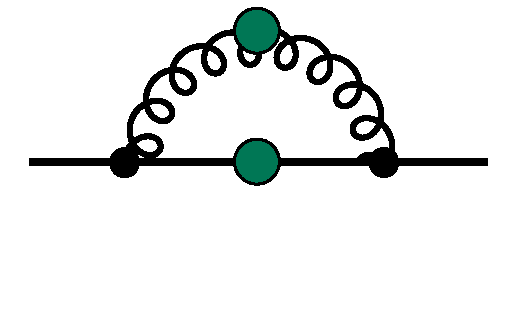
\includegraphics[scale=0.28, valign=c]{figs/diagrams/bphz/quark_self_energy_classical}\right]_{p=\mu}
\end{align*}

	\caption{Schematic spectral BPHZ-renormalization procedure at the example of the quark self energy diagram.} 
	\label{fig:BPHZ}
\end{figure}
\begin{itemize}
	\item  The diagram is subtracted by the first two terms of its own Taylor expansion around the RG scale $\mu$ in order to cancel quadratic and logarithmic divergences of the spectral integrands.\\[2em]
	\item This results in finite spectral integrands in the limit $\varepsilon\rightarrow 0$.
\end{itemize}
\end{frame}

\begin{frame}{Analytic Continuation of the finite Integrands}
\begin{itemize}
	\item Technical Detail: Split calculation of the diagram in Dirac vector and scalar part.
\end{itemize}
\begin{equation}
	\Sigma_q(p) =\slashed{p}\cdot\Sigma_{q}^D(p) + \Sigma_{q}^M(p),
\end{equation}
\begin{itemize}
	\item We are left with \alert{finite} spectral integrals:
\end{itemize}
\begin{align}
\Sigma_{q}^D(p) &= (-ig)^2\delta^{ab}C_f\int\limits_{\left\{\lambda_1,\lambda_2\right\}}\lambda_1\lambda_2\rho_A(\lambda_1)\rho_q^D(\lambda_2)\cdot I_q^D\left(p, \lambda_1, \lambda_2,x\right),\\
\Sigma_{q}^M(p) &= (-ig)^2\delta^{ab}C_f\int\limits_{\left\{\lambda_1,\lambda_2\right\}}\lambda_1\lambda_2\rho_A(\lambda_1)\rho_q^M(\lambda_2)\cdot I_q^M\left(p, \lambda_1, \lambda_2,x\right).
\end{align}
\begin{itemize}
	\item Analytic continuation to real frequencies according to
\end{itemize}
\begin{equation}
	I_q^{(D/M)}\left(\omega, \lambda_1, \lambda_2\right) := I_q^{(D/M)}\left(-i(\omega + i0^+)\right).
\end{equation}
\end{frame}

\begin{frame}{Iterative Solution of the Quark Propagator DSE}
\begin{figure}[t]
	%\centering
	\hspace{-2em}
	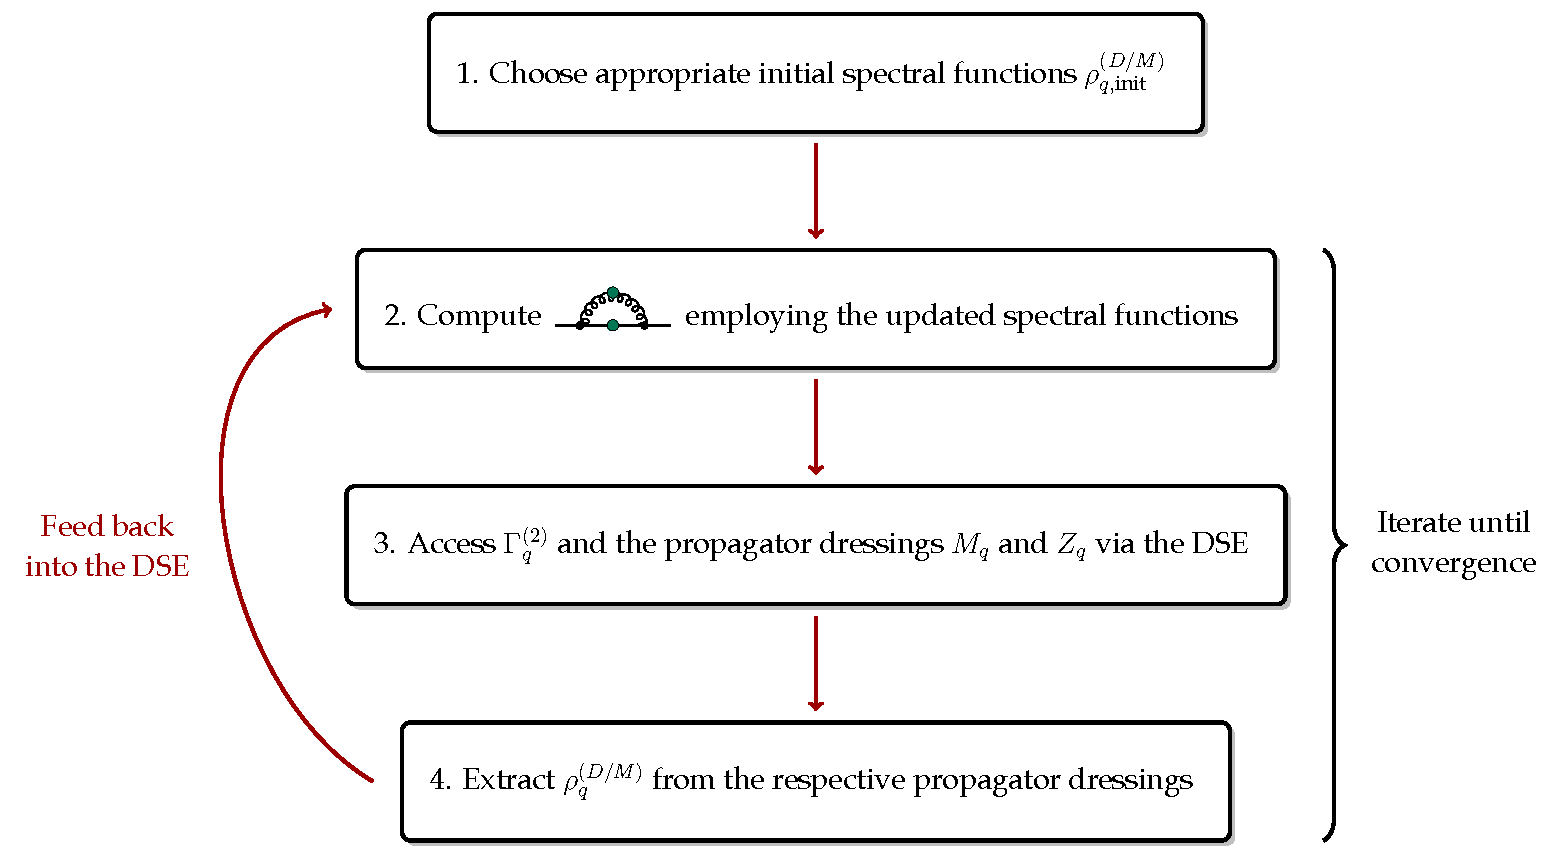
\includegraphics[width = 0.85\textwidth]{figs/tikz/iterative_computation}
\end{figure}
\end{frame}

\begin{frame}{Initial Setup: Gluon Spectral Function}
\begin{figure}[t]
\hfill
	\centering
	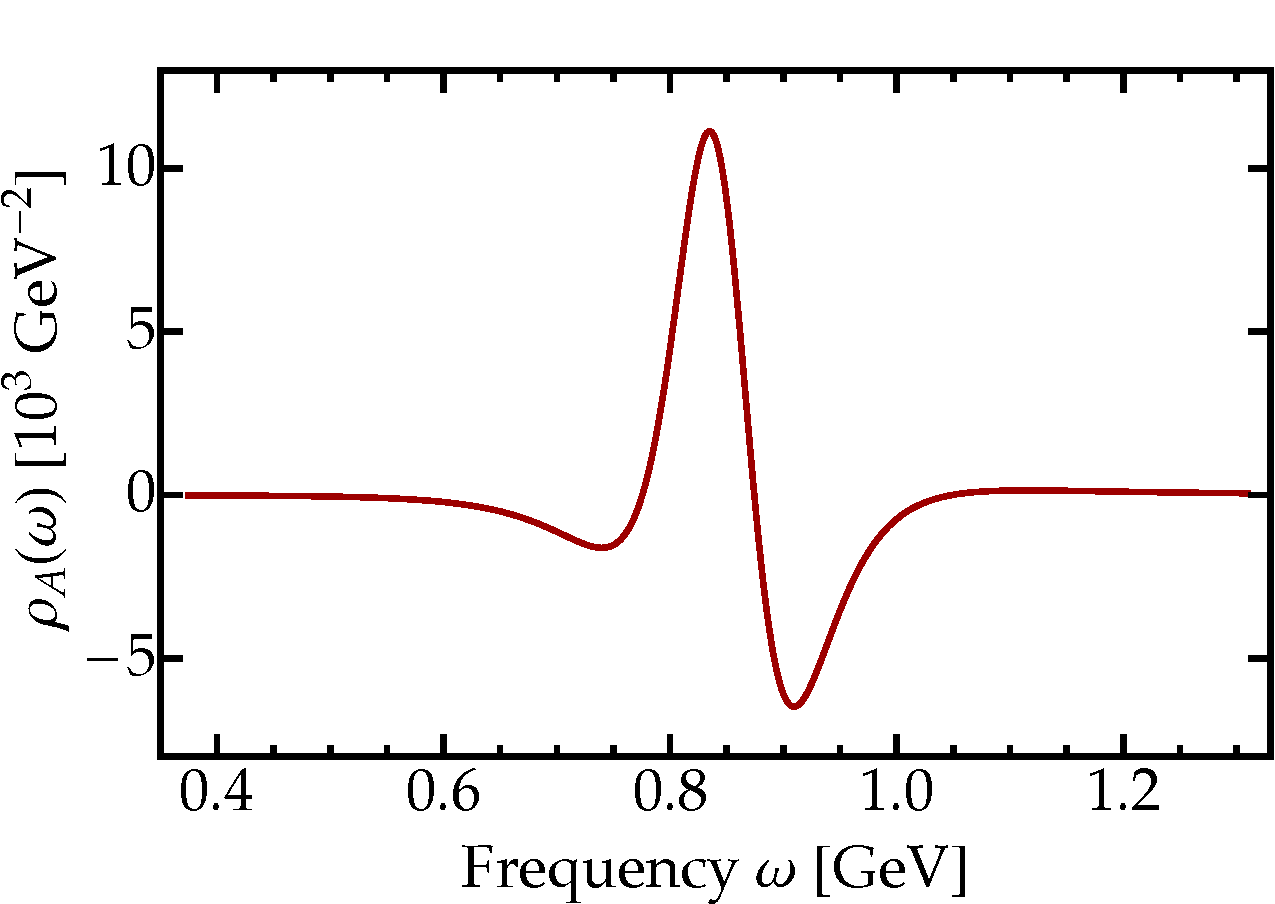
\includegraphics[width = 0.46\textwidth, trim= 4em 0 0 0]{figs/plots/GluonSpecFuncPlot}
\hfill
	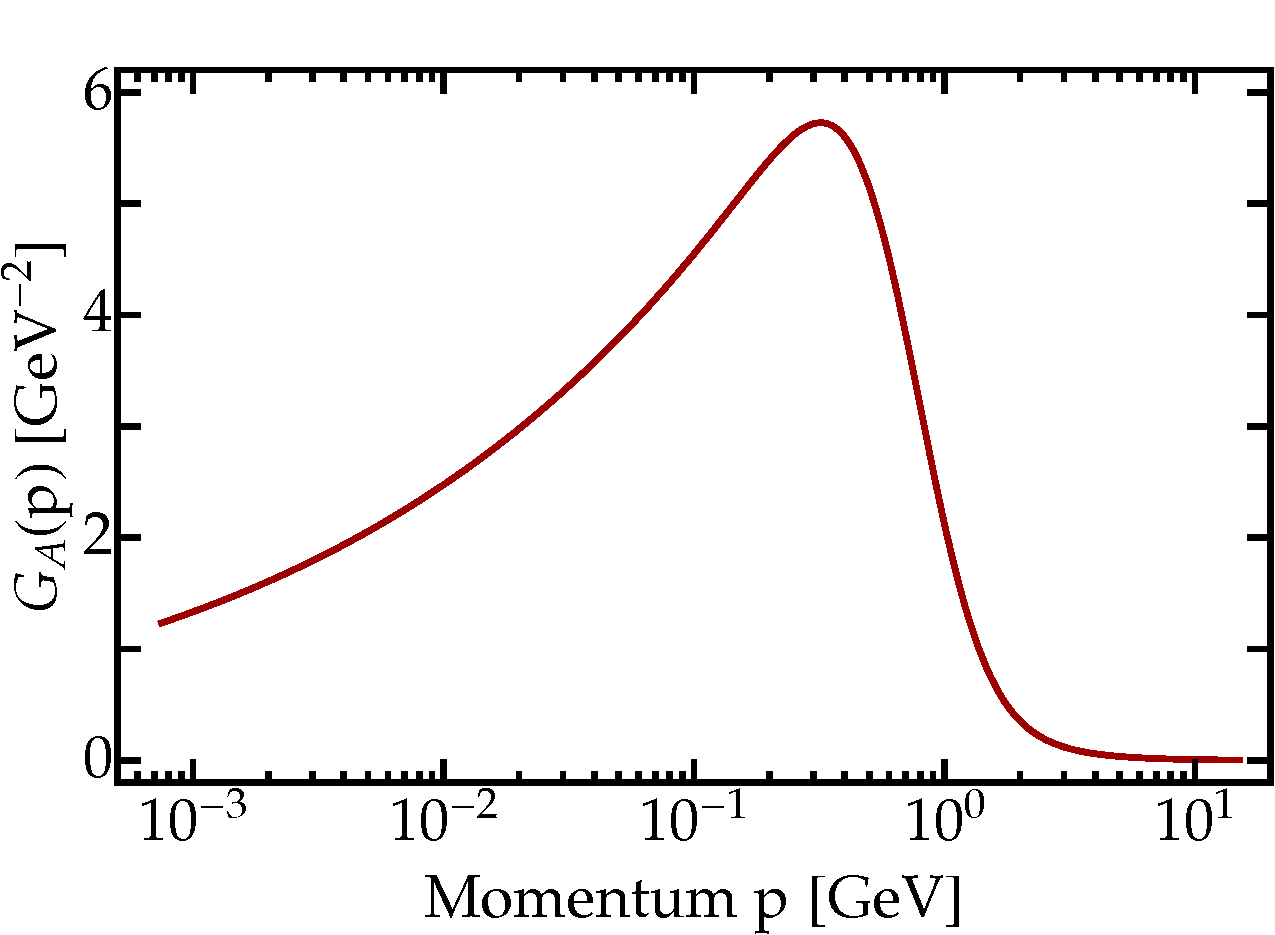
\includegraphics[width = 0.445\textwidth, trim= 4em 0 0 0]{figs/plots/GluonPropPlot}
\hfill
	\caption[Input gluon spectral function and corresponding propagator.]{Input gluon spectral function and corresponding propagator. Taken from arXiv:\alert{1804.00945}.}
\label{fig:gluon_specfunc_and_prop}
\end{figure}\end{frame}

\section{(Preliminary) Results}

\begin{frame}{Dressing Functions}
	\addtocounter{framenumber}{-1}
	 \begin{figure}[t] 
\hfill
	\centering
	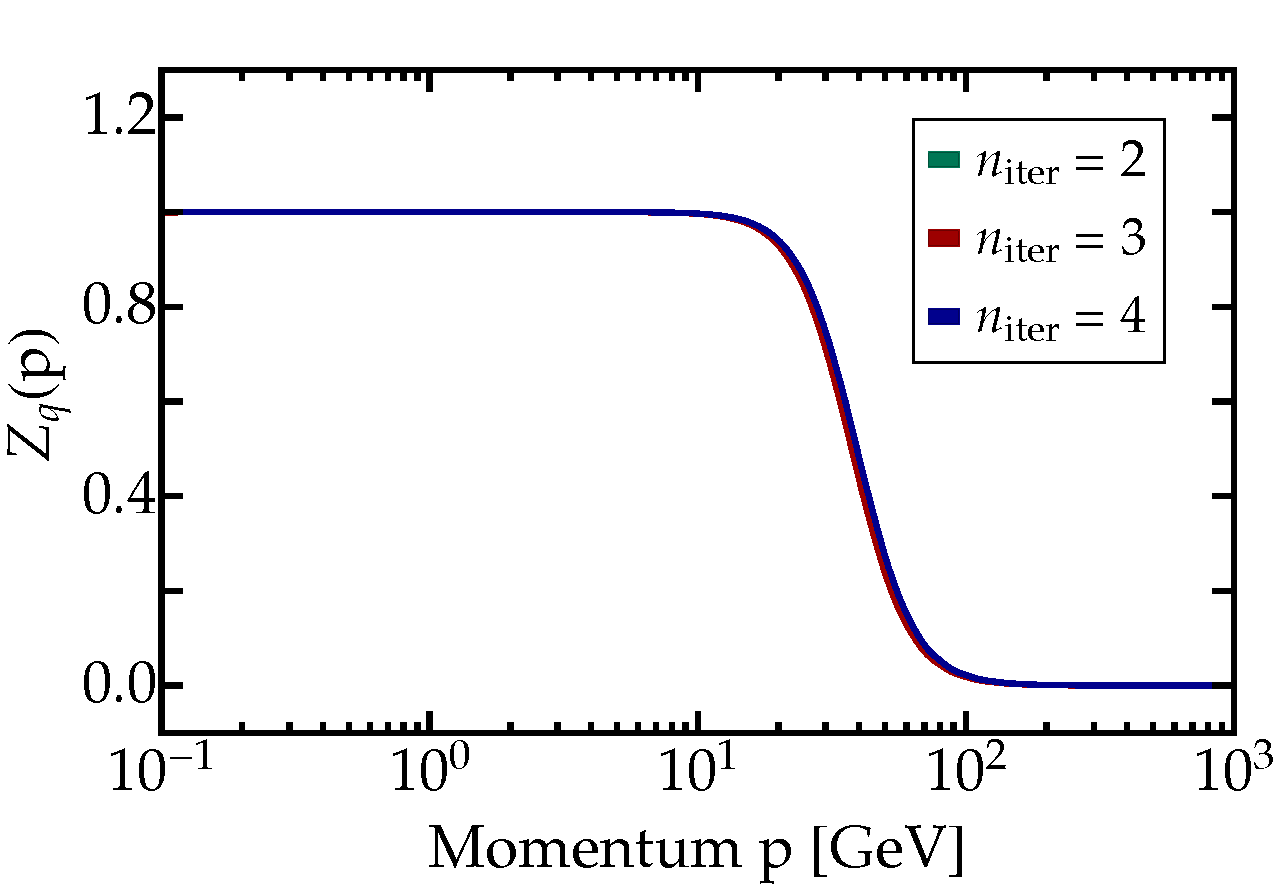
\includegraphics[width = 0.46\textwidth, trim= 4em 0 0 0]{figs/plots/ZqPlot}
\hfill
	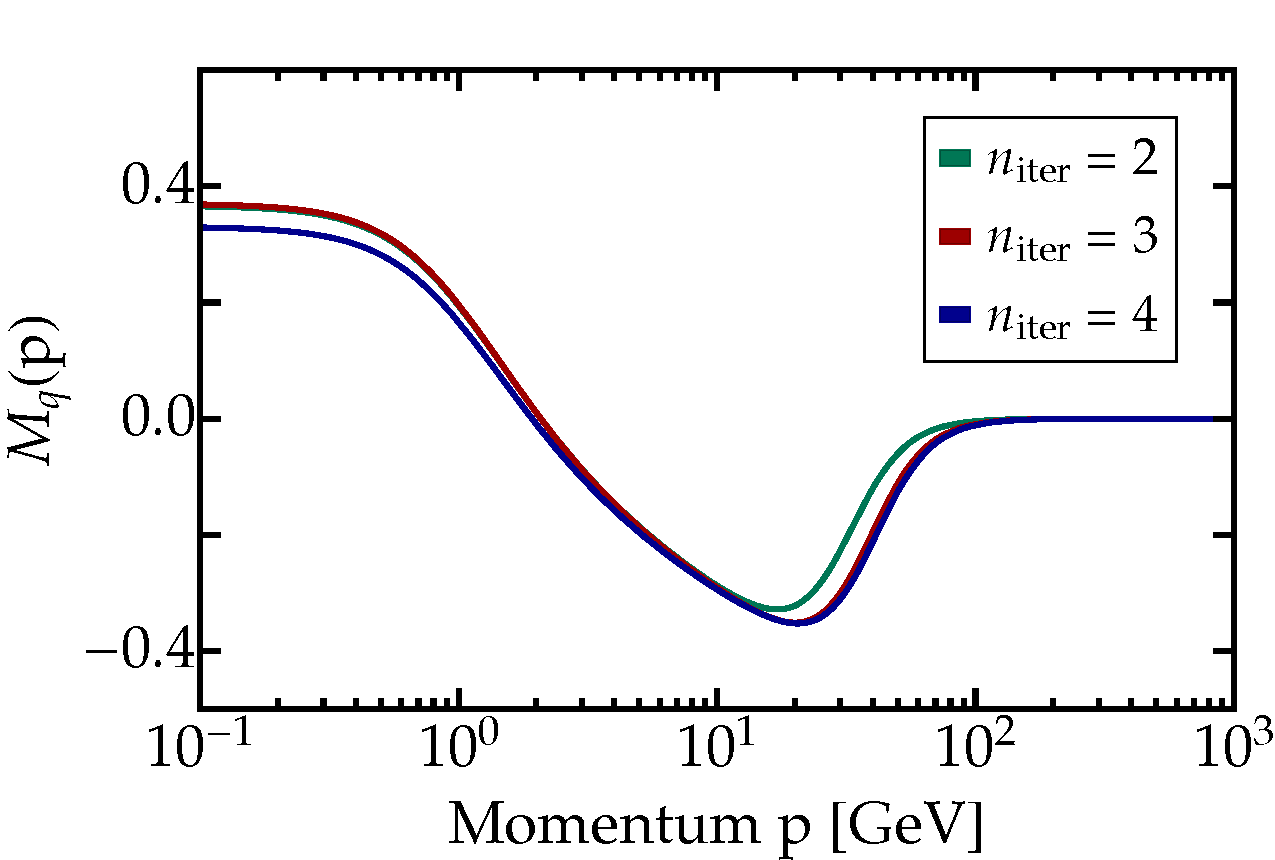
\includegraphics[width = 0.475\textwidth, trim= 4em 0 0 0]{figs/plots/MqPlot}
\hfill
	\caption[Computed quark propagator dressings $Z_q(p)$ and $M_q(p)$.]{Computed quark propagator dressings $Z_q(p)$ and $M_q(p)$ for different iteration steps.}
\label{fig:computed_dressings}
\end{figure}
\end{frame}

\begin{frame}{Quark Spectral Functions}
	 \begin{figure}[t] 
\hfill
	\centering
	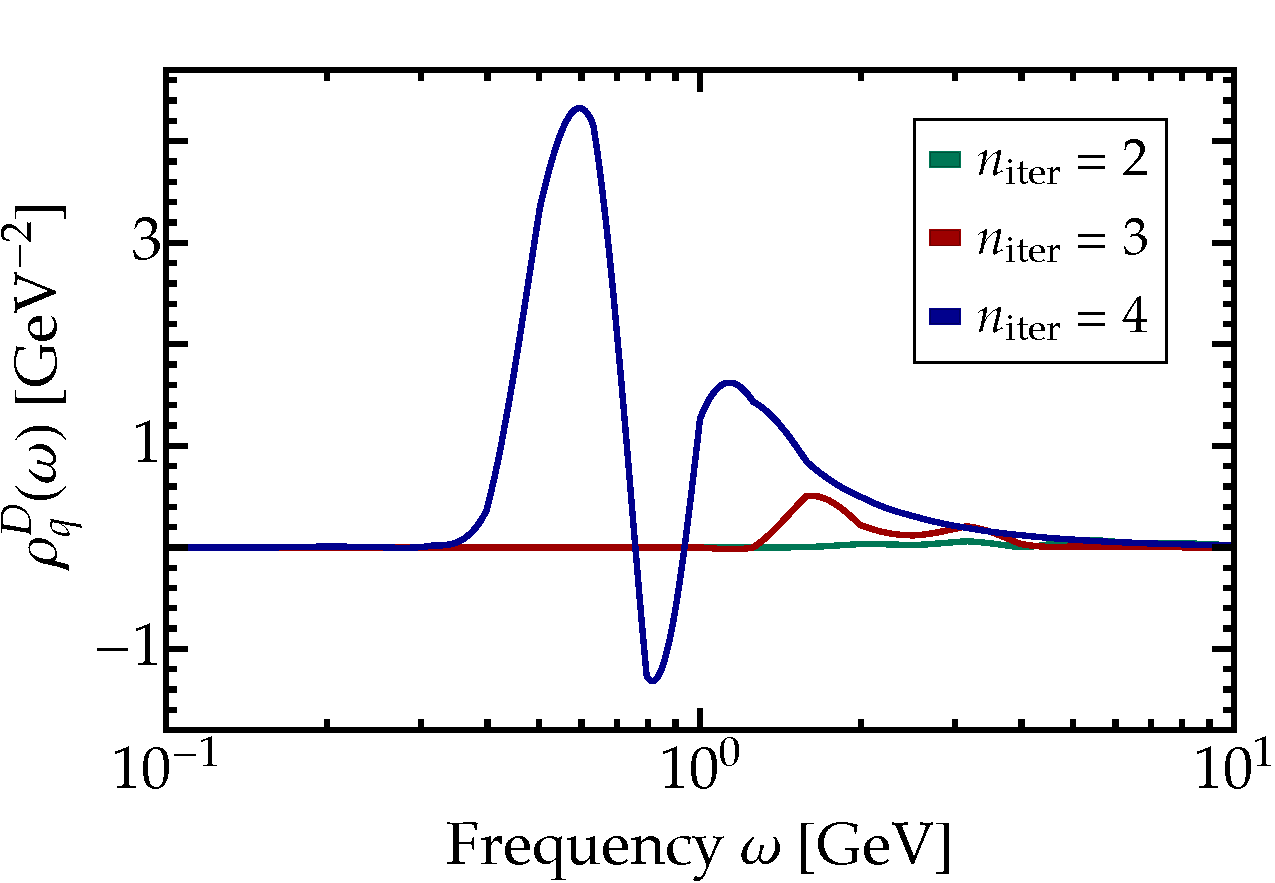
\includegraphics[width = 0.46\textwidth, trim= 4em 0 0 0]{figs/plots/rhoqDPlot}
\hfill
	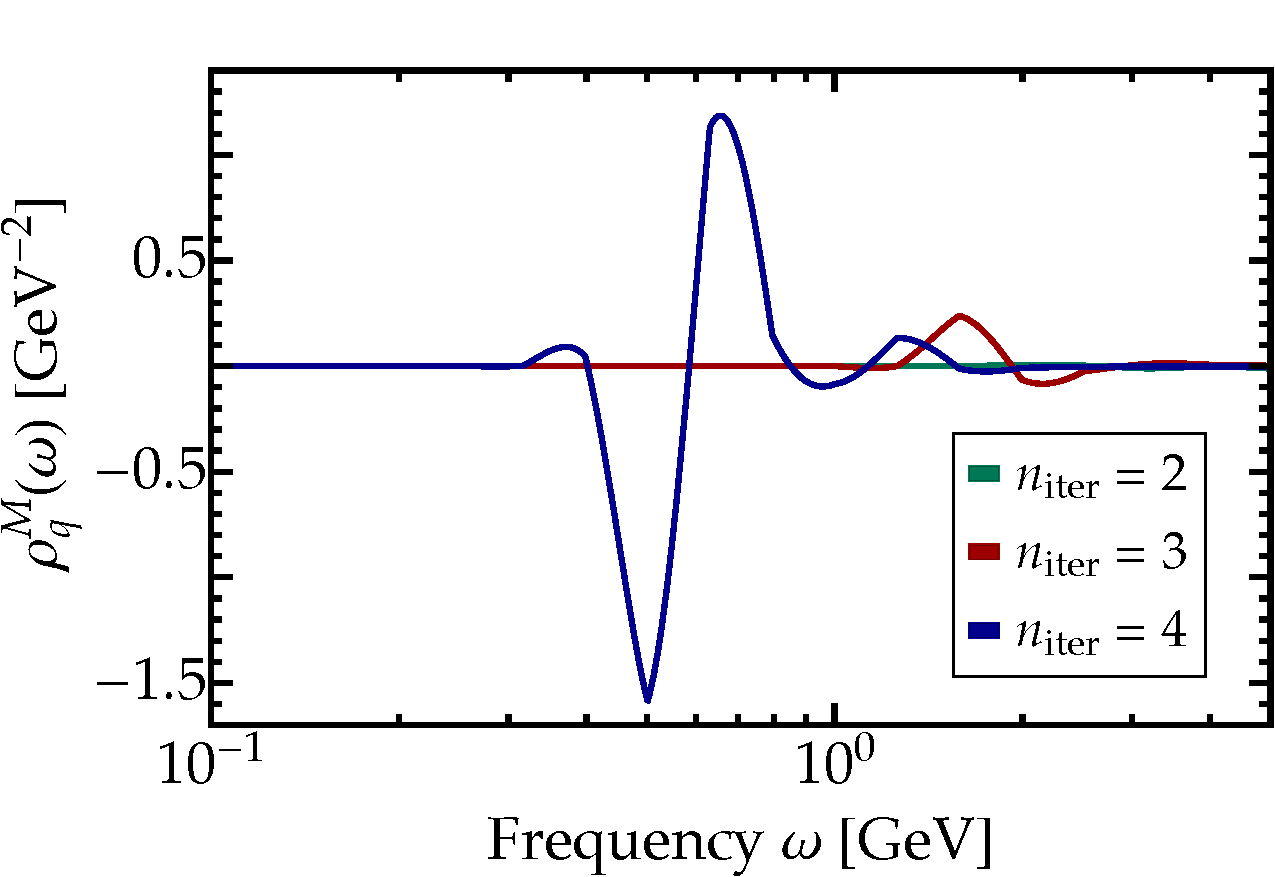
\includegraphics[width = 0.46\textwidth, trim= 4em 0 0 0 0]{figs/plots/rhoqMPlot}
\hfill 
	\caption{Computed quark spectral functions $\rho_q^D(\omega)$ and $\rho_q^M(\omega)$ for different numbers of iterations.
	}
\label{fig:specfunc_results}
\end{figure}

\end{frame}

\begin{frame}{Problem: Mismatch in the Comparison of the Euclidean Propagators}
	 \begin{figure}[t] 
\hfill
	\centering
	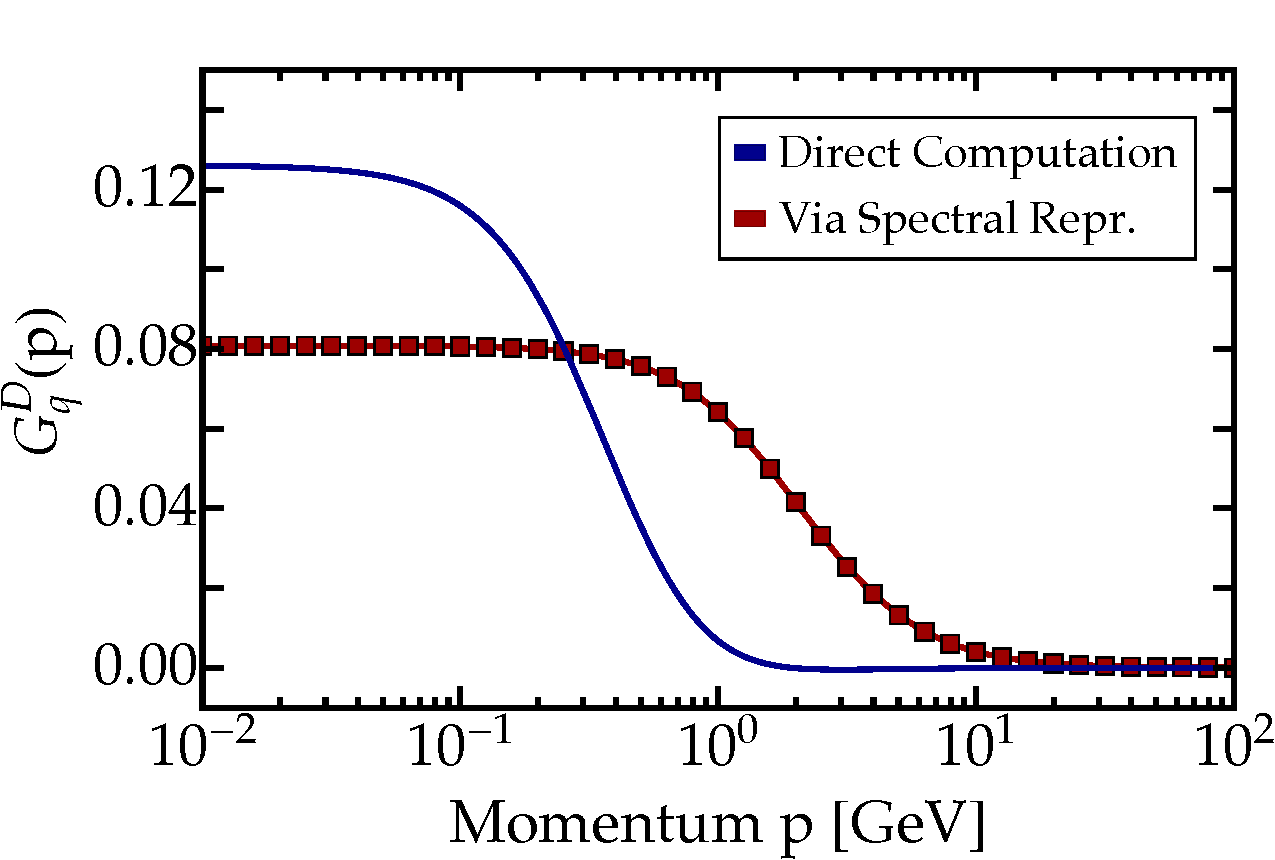
\includegraphics[width = 0.46\textwidth, trim= 4em 0 0 0]{figs/plots/BenchmarkPlotVec}
\hfill
	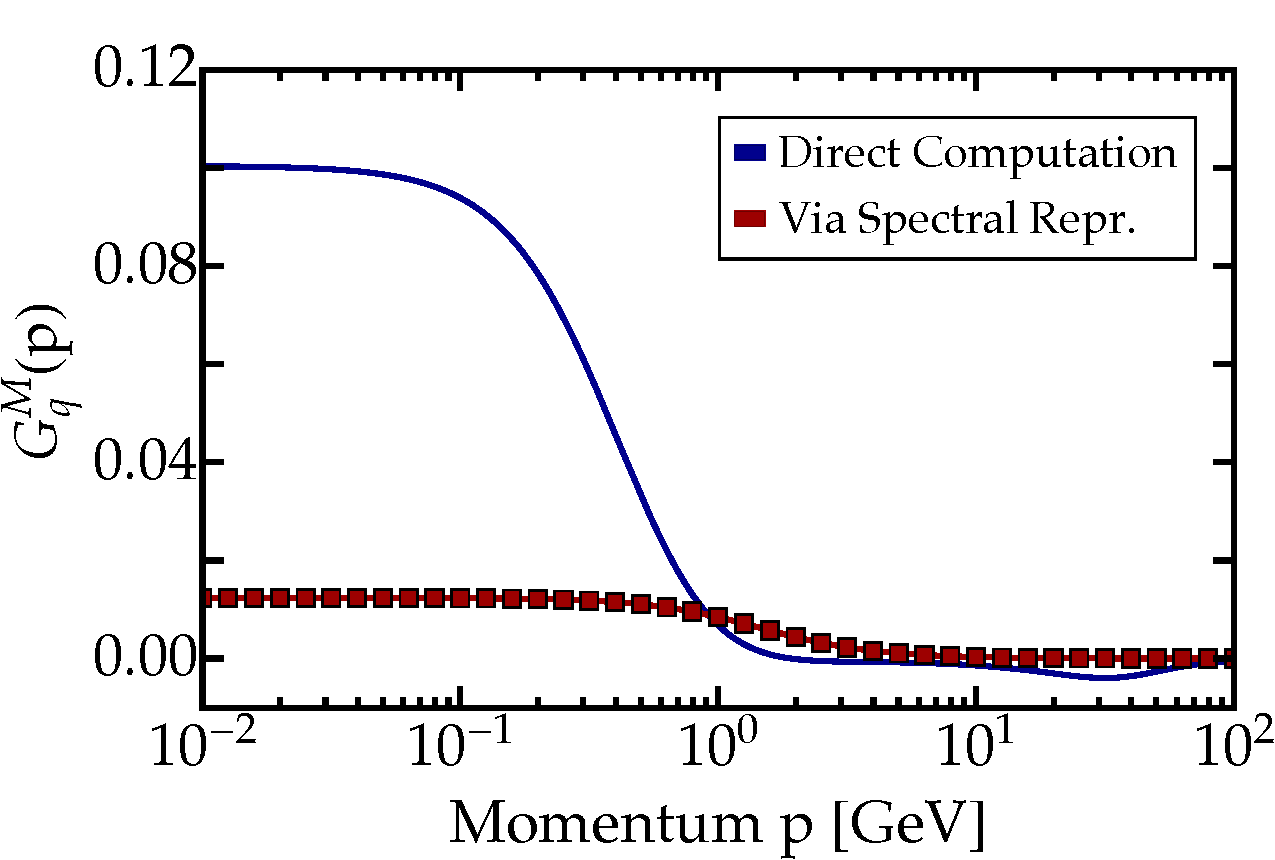
\includegraphics[width = 0.46\textwidth, trim= 4em 0 0 0 0]{figs/plots/BenchmarkPlotScal}
\hfill 
	\caption{Comparison of the respective parts of the Euclidean quark propagator with the result obtained from the spectral representation for the last iteration step $n_{\mathrm{iter}}=4$.}
\label{fig:specfunc_results}
\end{figure}
\end{frame}



\begin{frame}{Summary and Outlook}
\textbf{Current State of the Art:}
\begin{itemize}
	\item \alert{Spectral renormalization scheme} allows us to access (quark) spectral functions from the respective DSE
	\item Need to resolve mismatch in benchmark tests (Euclidean Propagators, Dressings, Perturbative expression for the Diagram ..)
\end{itemize}
\textbf{Next steps:}
\begin{itemize}
	\item Update Numerics: Avoid double counting of pole contribution, test different initial conditions, discretization \dots
\end{itemize}
\textbf{On longer terms:}
\begin{itemize}
	\item Full access to all QCD spectral functions ($\rightarrow$ Jan H., Nicolas, Julian et al.)
	\item Extend results to finite temperatures and densities ($\rightarrow$  Joschka)
	\item Access real-time dynamics of QCD
\end{itemize}
\end{frame}